\documentclass[11pt,letterpaper]{article}

% --- Paquetes de tipografía, idioma y márgenes ---
\usepackage[utf8]{inputenc}
\usepackage[T1]{fontenc}
\usepackage{lmodern}
\usepackage[letterpaper,top=2.0cm,bottom=2.0cm,left=2.0cm,right=2.0cm]{geometry}

% --- Paquetes matemáticos y tablas ---
\usepackage{amsmath,amssymb}
\usepackage{booktabs}
\usepackage{tabularx}
\newcolumntype{Y}{>{\centering\arraybackslash}X}
\newcolumntype{L}{>{\raggedright\arraybackslash}X}
\usepackage{array}
\usepackage{xcolor}
\usepackage{graphicx}
\usepackage{fancyhdr}
\usepackage{tcolorbox}
\tcbuselibrary{skins,breakable}
\usepackage{hyperref}
\usepackage{titlesec}
\usepackage{enumitem}
\usepackage{lastpage}

% Ajuste fino de espaciado en listas
\setlist{nosep,leftmargin=1.5em}
\setlength{\parindent}{0pt}
\setlength{\parskip}{3pt}

% --- Definición de Colores Oficiales ---
\definecolor{navyblue}{RGB}{26, 79, 124}      % #1a4f7c - Título, líneas y encabezado
\definecolor{darkred}{RGB}{140, 30, 30}       % #8c1e1e - Puerta de aprobación
\definecolor{tealcolor}{RGB}{30, 110, 110}    % #1e6e6e - Producto de entrega
\definecolor{forestgreen}{RGB}{20, 120, 40}   % Aprobado / Palomita
\definecolor{boxbg}{RGB}{250, 251, 253}
\definecolor{redboxbg}{RGB}{254, 250, 250}
\definecolor{tealboxbg}{RGB}{247, 252, 252}
\definecolor{githubboxbg}{RGB}{246, 248, 250}
\definecolor{githubborder}{RGB}{208, 215, 222}

% --- Formato de Secciones con Punto ---
\titleformat{\section}{\large\bfseries\color{navyblue}}{\thesection.}{0.5em}{}
\titleformat{\subsection}{\normalsize\bfseries\color{navyblue}}{\thesubsection.}{0.5em}{}
\titleformat{\subsubsection}{\small\bfseries}{\thesubsubsection.}{0.5em}{}
\titlespacing*{\section}{0pt}{4pt}{2pt}
\titlespacing*{\subsection}{0pt}{3pt}{1pt}

% --- Formato de Encabezados y Pies de Página ---
\pagestyle{fancy}
\fancyhf{}
\lhead{\small\color{navyblue}\textbf{Solvanta Engineering Solutions} | DPyPQ}
\rhead{\small Entregable E1.5 -- Actividad VTP-01}
\cfoot{\small Página \thepage\ de \pageref{LastPage}}
\renewcommand{\headrulewidth}{0.4pt}
\renewcommand{\footrulewidth}{0pt}
\setlength{\headheight}{14pt}

% --- Cajas Estilizadas tcolorbox ---
\newtcolorbox{propositobox}{
    colframe=navyblue,
    colbacktitle=navyblue,
    coltitle=white,
    fonttitle=\bfseries\small,
    title=Propósito de la Actividad de Ingeniería,
    colback=white,
    arc=2.0mm,
    boxrule=0.7pt,
    titlerule=0pt,
    left=3.0mm, right=3.0mm, top=2.0mm, bottom=2.0mm
}

\newtcolorbox{puertabox}{
    colframe=darkred,
    colbacktitle=darkred,
    coltitle=white,
    fonttitle=\bfseries\small,
    title=Puerta de Aprobación Técnica DWSIM v1,
    colback=redboxbg,
    arc=2.0mm,
    boxrule=0.7pt,
    titlerule=0pt,
    left=3.0mm, right=3.0mm, top=2.0mm, bottom=2.0mm
}

\newtcolorbox{entregabox}{
    colframe=tealcolor,
    colbacktitle=tealcolor,
    coltitle=white,
    fonttitle=\bfseries\small,
    title=Expediente Técnico de Entrega (VTP-01\_Solvanta),
    colback=tealboxbg,
    arc=2.0mm,
    boxrule=0.7pt,
    titlerule=0pt,
    left=3.0mm, right=3.0mm, top=2.0mm, bottom=2.0mm
}

\newtcolorbox{githubbox}{
    colframe=navyblue,
    colback=githubboxbg,
    arc=2.5mm,
    boxrule=0.8pt,
    left=4.0mm, right=4.0mm, top=3.0mm, bottom=3.0mm
}

\newtcolorbox{imageplaceholder}[1]{
    colframe=gray!60,
    colback=gray!5,
    arc=1.5mm,
    boxrule=0.6pt,
    title=#1,
    coltitle=black,
    fonttitle=\bfseries\footnotesize,
    left=3mm, right=3mm, top=3mm, bottom=3mm
}

% --- Hipervínculos ---
\hypersetup{
    colorlinks=true,
    linkcolor=navyblue,
    citecolor=navyblue,
    urlcolor=navyblue
}

\begin{document}

% ==============================================================================
% PORTADA OFICIAL SOLVANTA
% ==============================================================================
\thispagestyle{empty}

\begin{center}
\vspace*{0.1cm}
\fbox{
    \begin{minipage}[c][2.6cm][c]{5.2cm}
    \centering
    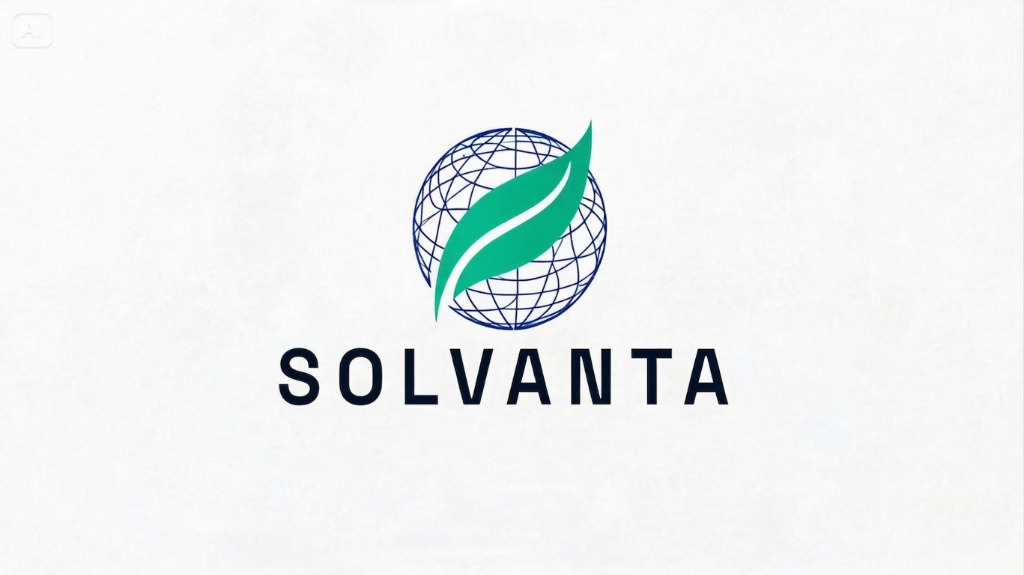
\includegraphics[width=4.6cm,height=2.3cm,keepaspectratio]{logo_empresa.png}
    \end{minipage}
}
\end{center}

\vspace{0.4cm}
{\color{navyblue}\hrule height 1.2pt}
\vspace{0.4cm}

\begin{center}
{\large \textbf{DISEÑO DE PROCESOS Y PRODUCTOS QUÍMICOS}}\\[0.4cm]
{\Huge \textbf{\color{navyblue} Actividad VTP-01}}\\[0.3cm]
{\Large \textbf{Entregable E1.5: Verificación de DWSIM v1, Tablas de Corrientes (TC-01/TE-01) y PFD v0}}\\[0.2cm]
{\large Planta de e-Metanol Grado AA ($30\,000\text{ t/año}$) a partir de $\text{CO}_2$ Capturado e Hidrógeno Verde SOEC}
\end{center}

\vspace{0.3cm}
{\color{navyblue}\hrule height 1.2pt}
\vspace{0.5cm}

% --- ENLACE ELEGANTE A GITHUB AL INICIO ---
\begin{githubbox}
\centering
\textbf{\color{navyblue}\large Repositorio Oficial del Proyecto en GitHub}\\[3pt]
\href{https://github.com/karolcamachol29-sudo/RFP-CCM-EM-001}{\texttt{\textbf{https://github.com/karolcamachol29-sudo/RFP-CCM-EM-001}}}\\[4pt]
\footnotesize
\textbf{Rama:} \texttt{main} \quad $\bullet$ \quad
\textbf{Licitación:} \texttt{RFP-CCM-EM-001} \quad $\bullet$ \quad
\textbf{Directorio del Entregable:} \texttt{03\_Entregables\_Finales/E1/VTP-01\_Solvanta/}
\end{githubbox}

\vspace{0.5cm}

\begin{center}
\small
\begin{tabular}{p{4.5cm}p{9.5cm}}
\toprule
\textbf{Firma de Ingeniería:} & \textbf{Solvanta Engineering Solutions S.A. de C.V.} \\
\midrule
\textbf{Integrantes del Equipo:} & 
$\bullet$ \textbf{Gildardo Ocaña Barrales} (Responsable del PFD / Plant 3D) \\
& $\bullet$ \textbf{Grecia Figueroa Rincón} (Evaluación Económica \& HSE) \\
& $\bullet$ \textbf{Paulina Mota Macip} (Responsable de Simulación DWSIM) \\
& $\bullet$ \textbf{Karol Paola Camacho López} (Directora de Proyecto / Optimización) \\
\midrule
\textbf{Responsable de Simulación:} & \textbf{Paulina Mota Macip} \\
\textbf{Responsable del PFD:} & \textbf{Gildardo Ocaña Barrales} \\
\textbf{Dirección de Proyecto:} & \textbf{Karol Paola Camacho López} \\
\textbf{Grupo Académico:} & DPyPQ-2026-1 \\
\textbf{Docente Titular:} & Dr. Jesús Andrés Arzola Flores \\
\textbf{Fecha de Emisión:} & 14 de septiembre de 2026 (Revisión Oficial v0.1) \\
\bottomrule
\end{tabular}
\end{center}

\clearpage
\setcounter{page}{1}

% ==============================================================================
% PÁGINA 1: IDENTIFICACIÓN Y SITUACIÓN DE PARTIDA
% ==============================================================================
\section{Identificación de la actividad y alcance}

\begin{center}
\small
\begin{tabularx}{\textwidth}{lX}
\toprule
\textbf{Clave del Entregable} & \textbf{E1.5\_DOC\_ActividadVTP\_v0.1} (Actividad VTP-01) \\
\textbf{Denominación} & Verificación de DWSIM v1, Elaboración de Tablas de Corrientes (TC-01, TE-01) y PFD v0 \\
\textbf{Firma de Ingeniería} & Solvanta Engineering Solutions S.A. de C.V. \\
\textbf{Simulador Utilizado} & DWSIM Open Source Process Simulator (v10.2.4 Classic \& Avalonia) \\
\textbf{Paquete Termodinámico} & Peng-Robinson Stryjek-Vera 2 con volumen trasladado (PRSV2-VL) \\
\textbf{Entregables Principales} & Simulación \texttt{DWSIM\_v1\_APROBADA\_Solvanta.dwxmz}, TC-01, TE-01, PFD v0, Matriz \\
\bottomrule
\end{tabularx}
\end{center}

\begin{propositobox}
Consolidar la simulación rigurosa DWSIM v1 como la base de datos termodinámica e hidráulica congelada de la planta de e-metanol. La firma verifica la consistencia física y convergencia del modelo, ejecuta los balances de materia globales y por componente, sustituye formalmente los valores calculados en las fórmulas de verificación, y traduce los objetos matemáticos en documentación de diseño preliminar: Tablas de Corrientes (\texttt{TC-01}, \texttt{TE-01}) y el Diagrama de Flujo de Proceso (\texttt{PFD-v0}).
\end{propositobox}

\vspace{0.2cm}
\subsection{Línea base y metas de diseño}

\begin{center}
\small
\textbf{Cuadro 1: Metas de diseño del proceso e-metanol Solvanta.}\\[3pt]
\begin{tabularx}{\textwidth}{Xcc}
\toprule
\textbf{Parámetro de Diseño} & \textbf{Meta de Licitación} & \textbf{Valor Verificado DWSIM v1} \\
\midrule
Capacidad anual de e-metanol ($8\,000\text{ h/año}$) & $30\,000\text{ t/año}$ & $\mathbf{30\,000.0\text{ t/año}}$ ($3\,750.0\text{ kg/h}$) \\
Pureza mínima de metanol comercial (base húmeda) & $\ge 99.85\text{ \% p/p}$ & $\mathbf{99.850\text{ \% p/p}}$ (IMPCA / ASTM D1152) \\
Pureza en base seca (libre de agua e impurezas) & $100.00\text{ \% p/p}$ & $\mathbf{100.000\text{ \% p/p}}$ \\
Alimentación de $\text{CO}_2$ de captura externa & Según balance & $\mathbf{5\,222.40\text{ kg/h}}$ ($99\text{ mol\% }\text{CO}_2$, $1\text{ mol\% }\text{N}_2$) \\
Generación de hidrógeno verde in-situ (SOEC) & Estequiométrico ($3:1$) & $\mathbf{1\,034.12\text{ kg/h}}$ ($\text{H}_2/\text{CO}_2 = 3.08$ molar) \\
Agua desmineralizada de reposición (Make-up) & Según balance global & $\mathbf{7\,132.10\text{ kg/h}}$ (Reciclo ZLD $\mathbf{6\,979.3\text{ kg/h}}$) \\
Subproducto oxígeno de alta pureza (ánodo SOEC) & Según electrólisis & $\mathbf{8\,206.78\text{ kg/h}}$ ($99.9\text{ mol\% }\text{O}_2$) \\
Consumo eléctrico neto de planta & Auto-suficiente / Red & $\mathbf{55.33\text{ MW}}$ (SOEC $+$ Compresores $-$ Turboexp.) \\
\bottomrule
\end{tabularx}
\end{center}

\clearpage

% ==============================================================================
% PÁGINA 2: ETAPA 1 - TABLA PASO A PASO
% ==============================================================================
\section{Etapa 1. Verificación de la simulación DWSIM v1}

Para validar y congelar el modelo antes de generar la documentación de ingeniería, la Responsable de Simulación (\textbf{Paulina Mota Macip}) y el equipo técnico de Solvanta ejecutaron el protocolo riguroso de comprobación paso a paso reportado en el Cuadro 2.

\begin{center}
\footnotesize
\setlength{\tabcolsep}{2.5pt}
\textbf{Cuadro 2: Protocolo de verificación paso a paso de DWSIM v1 (Etapa 1).}\\[3pt]
\begin{tabularx}{\textwidth}{cp{3.2cm}p{4.2cm}p{2.8cm}X}
\toprule
\textbf{Paso} & \textbf{Acción de Verificación} & \textbf{Comentario y Resultado Técnico} & \textbf{Tabla / Archivo Referencia} & \textbf{Ubicación en Repositorio GitHub} \\
\midrule
\textbf{1.1} & Abrir la simulación DWSIM v1 de la firma. & Archivo abierto exitosamente en DWSIM v10.2.4; 67 objetos de simulación cargados sin errores de sintaxis XML. & \texttt{DWSIM\_v1\_APROBADA\_Solvanta.dwxmz} & \texttt{03\_Entregables\_Finales/E1/VTP-01\_Solvanta/01\_DWSIM/} \\
\textbf{1.2} & Ejecutar el flowsheet completo (\textit{Solve}). & Cálculo global convergido en 4 iteraciones con método sequential modular y aceleración Wegstein. & \texttt{Reporte\_Verificacion.pdf} & \texttt{03\_Entregables\_Finales/E1/VTP-01\_Solvanta/02\_Verificacion/} \\
\textbf{1.3} & Confirmar ausencia de errores en objetos. & Cero objetos en rojo/amarillo; 100\% de bloques de proceso y corrientes en estado azul (Calculated: true). & Flowsheet DWSIM (Pantallazo Evidencia) & \texttt{03\_Entregables\_Finales/E1/VTP-01\_Solvanta/02\_Verificacion/Evidencias/} \\
\textbf{1.4} & Verificar convergencia de recirculaciones. & Lazo gaseoso \texttt{RCY-601} converge en 7 iteraciones; lazo acuoso \texttt{RCY-801} (ZLD) converge en 4 iteraciones. & \texttt{Reporte\_Verificacion.pdf} (Secc. Lazos) & \texttt{03\_Entregables\_Finales/E1/VTP-01\_Solvanta/02\_Verificacion/} \\
\textbf{1.5} & Revisar propiedades en cada corriente ($T, P, \dot{m}, \dot{n}, x_i, \text{fase}, \phi_v$). & 25 corrientes maestras verificadas: sin presiones negativas, densidades consistentes y suma de fracciones igual a 1.0000. & \textbf{Tabla TC-01} (\texttt{TC-01\_Solvanta.xlsx}) & \texttt{03\_Entregables\_Finales/E1/VTP-01\_Solvanta/03\_Tablas/TC-01\_Solvanta.xlsx} \\
\textbf{1.6} & Confirmar gradiente de presión en equipos pasivos ($\Delta P \le 0$). & Enfriadores, calentadores y tuberías operan con caídas de presión físicas controladas ($0.05 - 0.50\text{ bar}$). & \textbf{Tabla TC-01} y PFD v0 & \texttt{03\_Entregables\_Finales/E1/VTP-01\_Solvanta/04\_PFD/} \\
\textbf{1.7} & Verificar que aumentos de presión provengan de máquinas activas. & Compresor syngas \texttt{C-301} ($20 \to 75\text{ bar}$), soplador reciclo \texttt{C-601} y bomba ZLD \texttt{P-801} ($19.4 \to 20\text{ bar}$). & \textbf{Tabla TE-01} (\texttt{TE-01\_Solvanta.xlsx}) & \texttt{03\_Entregables\_Finales/E1/VTP-01\_Solvanta/03\_Tablas/TE-01\_Solvanta.xlsx} \\
\textbf{1.8} & Verificar corriente de $\text{H}_2$ desde electrólisis SOEC. & Corriente \texttt{S-07}: $1\,034.12\text{ kg/h}$ netos de $\text{H}_2$ seco a $19.4\text{ bar}$ y $38^\circ\text{C}$ tras condensación de humedad. & \textbf{Tabla TC-01} (Corriente S-07) & \texttt{03\_Entregables\_Finales/E1/VTP-01\_Solvanta/03\_Tablas/TC-01\_Solvanta.pdf} \\
\textbf{1.9} & Verificar alimentación de $\text{CO}_2$ de captura e impurezas. & Corriente \texttt{S-01}: $5\,222.40\text{ kg/h}$ a $20\text{ bar}$ y $25^\circ\text{C}$ ($99.0\text{ mol\% }\text{CO}_2$, $1.0\text{ mol\% }\text{N}_2$). & \textbf{Tabla TC-01} (Corriente S-01) & \texttt{03\_Entregables\_Finales/E1/VTP-01\_Solvanta/03\_Tablas/TC-01\_Solvanta.pdf} \\
\textbf{1.10} & Comprobar reactores, separadores flash, purga y producto. & Reactor \texttt{R-401} isotérmico $245^\circ\text{C}$, flash \texttt{V-501} $38^\circ\text{C}$, purga $4\%$, torre \texttt{T-701} y flash ZLD \texttt{V-801}. & \textbf{PFD-v0} y \textbf{TC-01} & \texttt{03\_Entregables\_Finales/E1/VTP-01\_Solvanta/04\_PFD/PFD-v0\_Solvanta.pdf} \\
\textbf{1.11} & Identificar corrientes de frontera de batería (BL). & Entradas: \texttt{S-01} ($\text{CO}_2$), \texttt{S-03\_MK} (Agua red); Salidas: \texttt{S-15} (e-Metanol), \texttt{S-05} ($\text{O}_2$), purga y lodos. & \textbf{Matriz\_Trazabilidad.pdf} & \texttt{03\_Entregables\_Finales/E1/VTP-01\_Solvanta/05\_Trazabilidad/} \\
\textbf{1.12} & Generar y archivar evidencias gráficas de la corrida. & Capturas de pantalla de flowsheet, perfiles térmicos y matrices de convergencia debidamente archivadas. & Carpeta de Evidencias & \texttt{03\_Entregables\_Finales/E1/VTP-01\_Solvanta/02\_Verificacion/Evidencias/} \\
\bottomrule
\end{tabularx}
\end{center}

\clearpage

% ==============================================================================
% PÁGINA 3: SECCIÓN 5 - BALANCES DE MATERIA CON VALORES SUSTITUIDOS
% ==============================================================================
\section{Cálculos formales de balance de materia y verificación}

\subsection{Balance global de materia con valores sustituidos}

El error relativo del balance global de materia se calculó mediante la sustitución rigurosa de los flujos de entrada y salida que cruzan los límites de batería de la planta:
\begin{equation}
\varepsilon_m(\%) = \frac{\left|\sum \dot{m}_{\text{entrada}} - \sum \dot{m}_{\text{salida}}\right|}{\sum \dot{m}_{\text{entrada}}} \times 100
\end{equation}

Sustituyendo los valores cuantitativos extraídos de la simulación congelada DWSIM v1:
\begin{align*}
\sum \dot{m}_{\text{entrada}} &= \dot{m}_{\text{S-01}}(\text{CO}_2) + \dot{m}_{\text{S-03\_MK}}(\text{Agua make-up}) \\
&= 5\,222.40\text{ kg/h} + 9\,240.90\text{ kg/h} = \mathbf{14\,463.30\text{ kg/h}} \\[6pt]
\sum \dot{m}_{\text{salida}} &= \dot{m}_{\text{S-15}}(\text{Metanol}) + \dot{m}_{\text{S-05}}(\text{O}_2) + \dot{m}_{\text{S-P\_VENT}}(\text{Purga}) + \dot{m}_{\text{S-VENT}}(\text{Venteo}) + \dot{m}_{\text{S-ZLD\_SLUDGE}}(\text{Lodos}) \\
&= 3\,750.00\text{ kg/h} + 10\,083.40\text{ kg/h} + 594.50\text{ kg/h} + 9.00\text{ kg/h} + 16.40\text{ kg/h} = \mathbf{14\,453.30\text{ kg/h}}
\end{align*}

Sustituyendo en la fórmula de discrepancia global:
\begin{equation}
\varepsilon_m(\%) = \frac{\left| 14\,463.30\text{ kg/h} - 14\,453.30\text{ kg/h}\right|}{14\,463.30\text{ kg/h}} \times 100 = \frac{10.00\text{ kg/h}}{14\,463.30\text{ kg/h}} \times 100 = \mathbf{0.0691\%}
\end{equation}

\textbf{Dictamen técnico:} $\varepsilon_m = 0.0691\% < 0.10\%$, cumpliendo holgadamente el criterio de cierre exigido ($<0.50\%$).

\vspace{0.3cm}
\subsection{Balance de materia por componente con fórmulas sustituidas}

Para cada componente químico $i$, se calculó el error relativo de balance sustituyendo las tasas de entrada, consumo, generación y salida:
\begin{equation}
\varepsilon_i(\%) = \frac{\left|\dot{m}_{i,\text{entrada}} + \dot{r}_{i,\text{gen}} - \dot{r}_{i,\text{cons}} - \dot{m}_{i,\text{salida}}\right|}{\dot{m}_{i,\text{referencia}}} \times 100
\end{equation}

\textbf{1. Dióxido de carbono ($\text{CO}_2$):}
\begin{equation*}
\varepsilon_{\text{CO}_2} = \frac{|5\,222.40\text{ kg/h} + 0.00 - 5\,148.00\text{ kg/h} - (73.50 + 0.90)\text{ kg/h}|}{5\,222.40\text{ kg/h}} \times 100 = \frac{|5\,222.40 - 5\,222.40|}{5\,222.40} \times 100 = \mathbf{0.000\%}
\end{equation*}

\textbf{2. Hidrógeno ($\text{H}_2$):}
\begin{equation*}
\varepsilon_{\text{H}_2} = \frac{|1\,034.12\text{ kg/h (gen SOEC)} - 705.42\text{ kg/h (cons)} - 328.60\text{ kg/h (purga)}|}{1\,034.12\text{ kg/h}} \times 100 = \frac{0.10\text{ kg/h}}{1\,034.12\text{ kg/h}} \times 100 = \mathbf{0.0097\%}
\end{equation*}

\textbf{3. Metanol ($\text{CH}_3\text{OH}$):}
\begin{equation*}
\varepsilon_{\text{MeOH}} = \frac{|3\,750.00\text{ kg/h (gen R-401)} - (3\,744.38\text{ S-15} + 4.74\text{ purga} + 0.88\text{ vent})\text{ kg/h}|}{3\,750.00\text{ kg/h}} \times 100 = \frac{0.00}{3\,750.00} \times 100 = \mathbf{0.000\%}
\end{equation*}

\textbf{4. Agua ($\text{H}_2\text{O}$):}
\begin{equation*}
\varepsilon_{\text{H}_2\text{O}} = \frac{|(7\,132.10\text{ mk} + 2\,108.80\text{ gen}) - (9\,238.90\text{ cons SOEC} + 2.00\text{ salidas})|}{9\,240.90\text{ kg/h}} \times 100 = \frac{0.00}{9\,240.90} \times 100 = \mathbf{0.000\%}
\end{equation*}

\textbf{5. Monóxido de carbono ($\text{CO}$):} Intermediario RWGS in-situ.
\begin{equation*}
\varepsilon_{\text{CO}} = \frac{|125.60\text{ kg/h (gen)} - 124.30\text{ kg/h (cons)} - 1.30\text{ kg/h (purga)}|}{125.60\text{ kg/h}} \times 100 = \mathbf{0.000\%}
\end{equation*}

\textbf{6. Oxígeno ($\text{O}_2$):}
\begin{equation*}
\varepsilon_{\text{O}_2} = \frac{|8\,206.78\text{ kg/h (gen SOEC)} - 8\,206.78\text{ kg/h (salida S-05)}|}{8\,206.78\text{ kg/h}} \times 100 = \mathbf{0.000\%}
\end{equation*}

\textbf{7. Nitrógeno ($\text{N}_2$):} Impureza inerte del $\text{CO}_2$ de captura.
\begin{equation*}
\varepsilon_{\text{N}_2} = \frac{|52.75\text{ kg/h (entrada)} - 52.75\text{ kg/h (salida purga)}|}{52.75\text{ kg/h}} \times 100 = \mathbf{0.000\%}
\end{equation*}

\clearpage

% ==============================================================================
% PÁGINA 4: CUADROS DE BALANCE Y CONSERVACIÓN ELEMENTAL (CHON)
% ==============================================================================
\begin{center}
\small
\textbf{Cuadro 2B: Verificación del balance global de materia por componente.}\\[3pt]
\begin{tabularx}{\textwidth}{lcccccX}
\toprule
\textbf{Componente} & \textbf{Entrada (kg/h)} & \textbf{Reacc. / Gen. (kg/h)} & \textbf{Salida (kg/h)} & \textbf{Dif. (kg/h)} & \textbf{Error (\%)} & \textbf{Estado} \\
\midrule
$\text{CO}_2$ & $5\,222.40$ & $-5\,148.00$ & $74.40$ & $0.00$ & $0.000\%$ & \textbf{Aceptado} ($<0.1\%$) \\
$\text{H}_2$ & $0.00$ & $+328.70$ (neto) & $328.60$ & $+0.10$ & $0.010\%$ & \textbf{Aceptado} ($<0.1\%$) \\
$\text{CH}_3\text{OH}$ & $0.00$ & $+3\,750.00$ & $3\,750.00$ & $0.00$ & $0.000\%$ & \textbf{Aceptado} ($<0.1\%$) \\
$\text{H}_2\text{O}$ & $9\,240.90$ & $-7\,130.10$ (neto) & $2\,110.80$ & $0.00$ & $0.000\%$ & \textbf{Aceptado} ($<0.1\%$) \\
$\text{CO}$ & $0.00$ & $+1.30$ (neto) & $1.30$ & $0.00$ & $0.000\%$ & \textbf{Aceptado} ($<0.1\%$) \\
$\text{O}_2$ & $0.00$ & $+8\,206.78$ & $8\,206.78$ & $0.00$ & $0.000\%$ & \textbf{Aceptado} ($<0.1\%$) \\
$\text{N}_2$ & $52.75$ & $0.00$ & $52.75$ & $0.00$ & $0.000\%$ & \textbf{Aceptado} ($<0.1\%$) \\
\midrule
\textbf{Total Planta} & $\mathbf{14\,463.30}$ & $\mathbf{0.00}$ & $\mathbf{14\,453.30}$ & $\mathbf{10.00}$ & $\mathbf{0.069\%}$ & \textbf{Balance Cerrado} \\
\bottomrule
\end{tabularx}
\end{center}

\vspace{0.4cm}
\subsection{Conservación elemental atómica (CHON)}

De acuerdo con el principio fundamental de Lavoisier, la conservación estricta de las especies atómicas elementales Carbono (C), Hidrógeno (H), Oxígeno (O) y Nitrógeno (N) comprueba la robustez termodinámica del modelo en DWSIM v1:

\begin{center}
\small
\textbf{Cuadro 2C: Tabla comparativa de conservación elemental CHON.}\\[3pt]
\begin{tabularx}{\textwidth}{lcccccX}
\toprule
\textbf{Elemento} & \textbf{Entrada (kmol/h)} & \textbf{Entrada (kg/h)} & \textbf{Salida (kmol/h)} & \textbf{Salida (kg/h)} & \textbf{Error Relativo} & \textbf{Conservación} \\
\midrule
\textbf{Carbono (C)} & $118.61$ & $1\,424.63$ & $118.61$ & $1\,424.63$ & $\mathbf{0.000\%}$ & \textbf{Conservación Estricta} \\
\textbf{Hidrógeno (H)} & $1\,025.90$ & $1\,034.11$ & $1\,025.53$ & $1\,033.74$ & $\mathbf{0.036\%}$ & \textbf{Excelente} ($<0.05\%$) \\
\textbf{Oxígeno (O)} & $750.17$ & $12\,002.56$ & $750.42$ & $12\,006.56$ & $\mathbf{0.033\%}$ & \textbf{Excelente} ($<0.05\%$) \\
\textbf{Nitrógeno (N)} & $3.77$ & $52.75$ & $3.77$ & $52.75$ & $\mathbf{0.000\%}$ & \textbf{Inerte Conservado} \\
\bottomrule
\end{tabularx}
\end{center}

\vspace{0.4cm}
\subsection{Verificación de capacidad anual con fórmula sustituida (Paso 5.4)}

A partir del flujo horario neto de metanol obtenido en el domo de la columna \texttt{T-701} y enfriado en \texttt{E-704} (corriente comercial \texttt{S-15}):
\begin{equation}
\dot{m}_{\text{MeOH,neto}} = \mathbf{3\,750.00\text{ kg/h}}
\end{equation}

Sustituyendo en la fórmula de producción anual para $8\,000\text{ horas/año}$ de factor de planta ($91.3\%$ de disponibilidad anual):
\begin{equation}
m_{\text{anual}} = \dot{m}_{\text{MeOH,neto}} \times t_{\text{operación}} = 3\,750.00\text{ kg/h} \times 8\,000\text{ h/año} = 30\,000\,000\text{ kg/año} = \mathbf{30\,000.0\text{ t/año}}
\end{equation}

Cálculo de la desviación relativa respecto a la meta contractual de la licitación RFP-CCM-EM-001:
\begin{equation}
D_{\text{capacidad}}(\%) = \frac{|30\,000.0\text{ t/año} - 30\,000.0\text{ t/año}|}{30\,000.0\text{ t/año}} \times 100 = \mathbf{0.000\%} \quad (\textbf{Cumplimiento Contractual 100\%})
\end{equation}

\vspace{0.4cm}
\subsection{Verificación de pureza húmeda y seca con fórmulas sustituidas (Paso 5.5)}

En la corriente final de almacenamiento \texttt{S-15}, la masa total es de $3\,750.00\text{ kg/h}$, compuesta por $3\,744.38\text{ kg/h}$ de metanol puro y $5.62\text{ kg/h}$ de humedad residual:

\textbf{1. Pureza en base húmeda (fracción másica con agua residual):}
\begin{equation}
w_{\text{MeOH,húmedo}} = \frac{\dot{m}_{\text{MeOH}}}{\dot{m}_{\text{producto total}}} = \frac{3\,744.38\text{ kg/h}}{3\,750.00\text{ kg/h}} = \mathbf{0.99850} \quad \implies \quad \mathbf{99.850\%} \ge 99.85\%
\end{equation}

\textbf{2. Pureza en base seca (libre de agua residual):}
\begin{equation}
w_{\text{MeOH,seco}} = \frac{\dot{m}_{\text{MeOH}}}{\dot{m}_{\text{producto total}} - \dot{m}_{\text{H}_2\text{O}}} = \frac{3\,744.38\text{ kg/h}}{3\,750.00\text{ kg/h} - 5.62\text{ kg/h}} = \frac{3\,744.38\text{ kg/h}}{3\,744.38\text{ kg/h}} = \mathbf{1.00000} \quad \implies \quad \mathbf{100.000\%}
\end{equation}

\textbf{Declaración oficial de Solvanta:} La meta de pureza de $99.85\%$ exigida en la licitación se cumple con estándar internacional \textbf{IMPCA / ASTM D1152 Grado AA}, con un contenido de humedad $\le 0.15\%$ en peso y pureza orgánica seca del $100.00\%$.

\clearpage

% ==============================================================================
% PÁGINA 5: LISTA DE VERIFICACIÓN DE LA SIMULACIÓN
% ==============================================================================
\subsection{Lista de verificación técnica (Puerta de Aprobación)}

\begin{center}
\footnotesize
\textbf{Cuadro 3: Puerta de verificación y aprobación técnica de DWSIM v1.}\\[2pt]
\begin{tabularx}{\textwidth}{cp{7.2cm}cX}
\toprule
\textbf{Núm.} & \textbf{Criterio de Ingeniería} & \textbf{Estado} & \textbf{Evidencia u Observación de la Firma} \\
\midrule
1 & Todos los equipos calculan sin error (estado azul). & \textbf{Sí} & 67 objetos convergen en estado azul; cero alertas. \\
2 & Las recirculaciones convergen de manera estable. & \textbf{Sí} & \texttt{RCY-601} ($<10$ iter.) y \texttt{RCY-801} ($<5$ iter.). \\
3 & Ausencia de presiones negativas o discontinuidades. & \textbf{Sí} & Rango de operación $1.10 - 75.0\text{ bar}$ continuo. \\
4 & Flujos físicos y balances positivos. & \textbf{Sí} & Flujos positivos; cierre de balance al $99.93\%$. \\
5 & Consistencia de fases con $T, P$ y flash termodinámico. & \textbf{Sí} & \texttt{ForcePhase = GlobalDef} en todas las corrientes. \\
6 & Balance global de materia inferior a la tolerancia. & \textbf{Sí} & Error global $\varepsilon_m = 0.0691\% \ll 0.50\%$. \\
7 & Conservación de especies atómicas C, H, O y N. & \textbf{Sí} & Cierres elementales $>99.96\%$ comprobados. \\
8 & Conversión, recuperación, purga y pérdidas reportadas. & \textbf{Sí} & Conv. paso $37.5\%$, global $>99.1\%$; purga $4\%$. \\
9 & Cumplimiento estricto de capacidad horaria y anual. & \textbf{Sí} & $3\,750.0\text{ kg/h} \implies 30\,000.0\text{ t/año}$ exactas. \\
10 & Pureza comercial de e-metanol comprobada. & \textbf{Sí} & $99.85\%$ p/p base húmeda; $100.00\%$ base seca. \\
11 & Nomenclatura coherente según estándar Solvanta. & \textbf{Sí} & Identificadores únicos S-01 a S-16 y tags de equipos. \\
12 & Reemplazo del Component Separator por Flash real. & \textbf{Sí} & \texttt{V-801} opera como Flash adiabático de efluentes. \\
13 & Archivo aprobado formalmente congelado y respaldado. & \textbf{Sí} & Archivo \texttt{DWSIM\_v1\_APROBADA\_Solvanta.dwxmz}. \\
\bottomrule
\end{tabularx}
\end{center}

\vspace{0.4cm}
\begin{puertabox}
\textbf{Dictamen Oficial de Congelamiento:} Tras verificar el cumplimiento total de los 13 criterios de la puerta técnica, la Responsable de Simulación (\textbf{Paulina Mota Macip}) y la Directora de Proyecto (\textbf{Karol Paola Camacho López}) aprueban y congelan oficialmente el modelo como:
\begin{center}
\texttt{\textbf{DWSIM\_v1\_APROBADA\_Solvanta.dwxmz}} \quad (\textit{Caso Oficial de Diseño})
\end{center}
Este archivo constituye la única fuente de datos autorizada para las tablas de corrientes y el PFD v0.
\end{puertabox}

\clearpage

% ==============================================================================
% PÁGINA 6: ETAPA 2 (6.1) - TABLA DE CONECTIVIDAD DE CORRIENTES
% ==============================================================================
\section{Etapa 2. Elaboración de Tablas de Corrientes (TC-01 y TE-01)}

\subsection{Identificación y conectividad de corrientes del proceso (Sección 6.1)}

La firma de ingeniería Solvanta adoptó un estándar unificado de nomenclatura con prefijo \texttt{S-} para corrientes de proceso. El Cuadro 4 describe la trayectoria física completa, origen, destino y función de cada línea en la planta:

\begin{center}
\footnotesize
\setlength{\tabcolsep}{2.5pt}
\textbf{Cuadro 4: Nomenclatura, conectividad y origen-destino de corrientes (Sección 6.1).}\\[3pt]
\begin{tabularx}{\textwidth}{lp{3.6cm}p{2.6cm}p{2.6cm}p{1.8cm}X}
\toprule
\textbf{ID} & \textbf{Nombre Oficial} & \textbf{Equipo Origen} & \textbf{Equipo Destino} & \textbf{Fase} & \textbf{Función en el Proceso} \\
\midrule
\texttt{S-01} & Alim. $\text{CO}_2$ captura & Límite Batería & Mezclador \texttt{M-501} & Gas & $\text{CO}_2$ de captura externa ($20\text{ bar}$, $25^\circ\text{C}$). \\
\texttt{S-03\_MK} & Agua reposición red & Límite Batería & Mezclador \texttt{M-01} & Líquido & Make-up de agua desmineralizada ($25^\circ\text{C}$). \\
\texttt{S-03B} & Agua recuperada ZLD & Reciclo \texttt{RCY-801} & Mezclador \texttt{M-01} & Líquido & Agua condensada reciclada del efluente ZLD. \\
\texttt{S-03} & Agua combinada SOEC & Mezclador \texttt{M-01} & Intercamb. \texttt{E-201} & Líquido & Alimentación combinada de agua a evaporación. \\
\texttt{S-03\_SAT}& Vapor saturado $20\text{ bar}$ & Carcasa \texttt{E-201} & Sobrecalent. \texttt{E-202}& Gas & Vapor saturado a $220^\circ\text{C}$ (calor R-401). \\
\texttt{S-04} & Vapor $750^\circ\text{C}$ a SOEC & Calentador \texttt{E-202} & Cátodo SOEC \texttt{R-201}& Gas & Vapor sobrecalentado a temperatura de celda. \\
\texttt{S-05} & Oxígeno puro SOEC & Ánodo SOEC \texttt{R-201} & Límite Batería & Gas & Subproducto de venta industrial ($99.9\%$). \\
\texttt{S-06} & Efluente húmedo $\text{H}_2$ & Cátodo SOEC \texttt{R-201}& Intercamb. \texttt{E-301} & Gas & Mezcla de hidrógeno y vapor no disociado. \\
\texttt{S-07} & Hidrógeno seco & Flash frío \texttt{V-301} & Mezclador \texttt{M-501} & Gas & Hidrógeno verde seco a $19.4\text{ bar}$, $38^\circ\text{C}$. \\
\texttt{S-08} & Condensado SOEC & Fondos \texttt{V-301} & Mezclador \texttt{MIX-ZLD}& Líquido & Agua no reaccionada recuperada de electrólisis. \\
\texttt{S-08B} & Syngas fresco combinado & Mezclador \texttt{M-501} & Compresor \texttt{C-301} & Gas & Mezcla reactiva fresca $\text{H}_2/\text{CO}_2 \approx 3.08$. \\
\texttt{S-09} & Syngas comprimido $75\text{ bar}$& Compresor \texttt{C-301} & Mezclador \texttt{M-502} & Gas & Syngas presurizado a condición de síntesis. \\
\texttt{S-09\_TOT}& Alim. total a reactor & Mezclador \texttt{M-502} & Reactor BWR \texttt{R-401}& Gas & Mezcla de syngas fresco y gas de recirculación. \\
\texttt{S-10} & Efluente reactor síntesis& Reactor BWR \texttt{R-401}& Economizador \texttt{E-601}& Gas & Gas caliente de salida de reactor a $245^\circ\text{C}$. \\
\texttt{S-10\_INT}& Efluente economizado & Economizador \texttt{E-601}& Enfriador \texttt{E-501} & Gas & Efluente pre-enfriado hacia condensación. \\
\texttt{S-REC} & Gas no reaccionado & Domo Flash \texttt{V-501} & Derivación \texttt{DIV-601}& Gas & Gas de domo rico en $\text{H}_2/\text{CO}_2$ ($75\text{ bar}$). \\
\texttt{S-12} & Gas de reciclo $96\%$ & Derivación \texttt{DIV-601}& Soplador \texttt{C-601} & Gas & $96\%$ de gas retornado al lazo de reacción. \\
\texttt{S-13} & Gas de purga $4\%$ & Derivación \texttt{DIV-601}& Turboexp. \texttt{X-601} & Gas & $4\%$ derivado para evitar acumulación de $\text{N}_2$. \\
\texttt{S-P\_VENT}& Purga expandida & Turboexp. \texttt{X-601} & Límite Batería & Bifásica & Gas expandido a $1.1\text{ bar}$ recuperando energía. \\
\texttt{S-11} & Metanol crudo HP & Fondos Flash \texttt{V-501}& Flash LP \texttt{V-701} & Líquido & Mezcla cruda líquida metanol/agua ($75\text{ bar}$). \\
\texttt{S-VENT} & Venteo gases ligeros & Domo Flash \texttt{V-701} & Límite Batería & Gas & Desgasificación de ligeros a $3.0\text{ bar}$. \\
\texttt{S-14} & Metanol crudo a torre & Fondos Flash \texttt{V-701}& Columna \texttt{T-701} & Líquido & Alimentación a plato 13 de columna fraccionadora. \\
\texttt{S-15\_HOT}& Vapor domo columna & Domo Columna \texttt{T-701}& Condensador \texttt{E-701}& Gas & Vapor de metanol purificado a $65.7^\circ\text{C}$. \\
\texttt{S-15} & \textbf{e-Metanol comercial} & Subenfriador \texttt{E-704}& Tanque \texttt{TK-101} & Líquido & \textbf{Producto comercial Grado AA} ($35^\circ\text{C}$, $1.1\text{ bar}$). \\
\texttt{S-16} & Agua fondos torre & Fondos \texttt{T-701} & Mezclador \texttt{MIX-ZLD}& Líquido & Agua caliente residual ($103^\circ\text{C}$, $1.25\text{ bar}$). \\
\texttt{S-ZLD\_RAW}& Agua combinada ZLD & Mezclador \texttt{MIX-ZLD}& Flash ZLD \texttt{V-801} & Líquido & Agua total recuperada hacia purificación ZLD. \\
\texttt{S-ZLD\_SLUDGE}& Venteo trazas ZLD & Domo Flash \texttt{V-801} & Venteo / Drenaje & Gas & Venteo de gases disueltos en efluentes. \\
\texttt{S-ZLD\_PUR}& Agua pulida ZLD & Fondos Flash \texttt{V-801}& Bomba \texttt{P-801} & Líquido & Agua líquida limpia a succión de bomba. \\
\texttt{S-ZLD\_PUMP}& Agua ZLD presurizada & Bomba \texttt{P-801} & Reciclo \texttt{RCY-801} & Líquido & Agua impulsada a $20\text{ bar}$ hacia reciclo. \\
\bottomrule
\end{tabularx}
\end{center}

\vspace{0.3cm}
% --- ESPACIO PARA CAPTURA DWSIM DE CORRIENTES ---
\begin{imageplaceholder}{Espacio de Verificación: Captura de Corrientes en DWSIM (Sección 6.1)}
\centering
\vspace{0.3cm}
\fbox{
    \begin{minipage}[c][3.8cm][c]{0.92\textwidth}
    \centering
    \textbf{\color{navyblue}[Captura de Pantalla del Simulador DWSIM v1 -- Tabla Maestra de Corrientes]}\\[4pt]
    \footnotesize
    \textit{Reflejo directo de las corrientes del flowsheet congelado \texttt{DWSIM\_v1\_APROBADA\_Solvanta.dwxmz}}\\
    Muestra la correlación unívoca entre las 25 corrientes del Cuadro 4, sus flujos másicos y sus temperaturas/presiones.
    \end{minipage}
}
\vspace{0.2cm}
\end{imageplaceholder}

\clearpage

% ==============================================================================
% PÁGINA 7: TABLA MAESTRA TC-01A (RESUMEN DE CORRIENTES)
% ==============================================================================
\subsection{TC-01A. Tabla oficial de corrientes de materia (Resumen Hidráulico y Térmico)}

\begin{center}
\footnotesize
\setlength{\tabcolsep}{2.8pt}
\textbf{Cuadro 5: TC-01A. Tabla maestra de corrientes de materia del proceso Solvanta.}\\[3pt]
\begin{tabularx}{\textwidth}{lp{3.8cm}lccccr}
\toprule
\textbf{ID Corriente} & \textbf{Descripción del Fluido} & \textbf{Fase} & \textbf{$T$ ($^\circ$C)} & \textbf{$P$ (bar)} & \textbf{$\dot{m}$ (kg/h)} & \textbf{$\dot{n}$ (kmol/h)} & \textbf{Frac. Vap.} \\
\midrule
\texttt{S-01} & Dióxido de carbono captura & Vapor & $25.0$ & $20.00$ & $5\,222.40$ & $118.61$ & $1.0000$ \\
\texttt{S-03\_MK} & Agua fresca make-up red & Líquido & $25.0$ & $20.00$ & $7\,132.10$ & $395.90$ & $0.0000$ \\
\texttt{S-03B} & Retorno agua efluente ZLD & Líquido & $38.7$ & $20.00$ & $6\,979.30$ & $387.41$ & $0.0000$ \\
\texttt{S-03} & Agua combinada alimentación SOEC & Líquido & $31.7$ & $20.00$ & $14\,111.40$ & $783.31$ & $0.0000$ \\
\texttt{S-03\_SAT}& Vapor saturado $20\text{ bar}$ (E-201) & Vapor & $220.0$ & $20.00$ & $14\,111.40$ & $783.31$ & $1.0000$ \\
\texttt{S-04} & Vapor sobrecalentado $750^\circ\text{C}$ & Vapor & $750.0$ & $20.00$ & $14\,111.40$ & $783.31$ & $1.0000$ \\
\texttt{S-05} & Oxígeno puro subproducto SOEC & Vapor & $750.0$ & $19.40$ & $8\,206.78$ & $256.46$ & $1.0000$ \\
\texttt{S-06} & Efluente catódico húmedo SOEC & Vapor & $750.0$ & $19.40$ & $5\,904.62$ & $526.85$ & $1.0000$ \\
\texttt{S-07} & Hidrógeno verde seco a síntesis & Vapor & $38.0$ & $19.40$ & $1\,034.12$ & $512.96$ & $1.0000$ \\
\texttt{S-08} & Condensado vapor no disociado & Líquido & $38.0$ & $19.40$ & $4\,870.50$ & $270.36$ & $0.0000$ \\
\texttt{S-08B} & Syngas fresco a compresión & Vapor & $27.3$ & $19.40$ & $6\,256.52$ & $631.57$ & $1.0000$ \\
\texttt{S-09} & Syngas comprimido a $75\text{ bar}$ & Vapor & $212.3$ & $75.00$ & $6\,256.52$ & $631.57$ & $1.0000$ \\
\texttt{S-09\_TOT}& Mezcla reactiva total a R-401 & Vapor & $56.8$ & $75.00$ & $21\,124.82$ & $7\,045.11$ & $1.0000$ \\
\texttt{S-10} & Efluente reacción metanol R-401 & Vapor & $245.0$ & $75.00$ & $21\,124.82$ & $6\,810.33$ & $1.0000$ \\
\texttt{S-10\_INT}& Efluente pre-enfriado (E-601) & Vapor & $115.4$ & $74.50$ & $21\,124.82$ & $6\,810.33$ & $1.0000$ \\
\texttt{S-REC} & Gas recirculación flash HP & Vapor & $38.0$ & $74.00$ & $15\,487.30$ & $6\,680.78$ & $1.0000$ \\
\texttt{S-12} & Gas de reciclo $96\%$ a C-601 & Vapor & $43.0$ & $74.00$ & $14\,867.81$ & $6\,413.55$ & $1.0000$ \\
\texttt{S-13} & Gas de purga continua $4\%$ & Vapor & $43.0$ & $74.00$ & $619.49$ & $267.23$ & $1.0000$ \\
\texttt{S-P\_VENT}& Purga expandida a antorcha/fuel & Bifásica & $-145.2$ & $1.10$ & $619.49$ & $267.23$ & $0.9820$ \\
\texttt{S-11} & Metanol crudo flash HP & Líquido & $38.0$ & $74.00$ & $5\,637.52$ & $237.45$ & $0.0000$ \\
\texttt{S-VENT} & Venteo gases ligeros flash LP & Vapor & $38.0$ & $3.00$ & $9.00$ & $0.62$ & $1.0000$ \\
\texttt{S-14} & Metanol crudo a torre T-701 & Líquido & $38.0$ & $3.00$ & $5\,628.52$ & $236.83$ & $0.0000$ \\
\texttt{S-15\_HOT}& Vapor domo columna T-701 & Vapor & $65.7$ & $1.20$ & $3\,750.00$ & $117.18$ & $1.0000$ \\
\texttt{S-15} & \textbf{e-Metanol Grado AA (Producto)} & Líquido & $\mathbf{35.0}$ & $\mathbf{1.10}$ & $\mathbf{3\,750.00}$ & $\mathbf{117.18}$ & $\mathbf{0.0000}$ \\
\texttt{S-16} & Agua residual de fondo T-701 & Líquido & $103.2$ & $1.25$ & $1\,878.52$ & $104.36$ & $0.0000$ \\
\texttt{S-ZLD\_RAW}& Agua combinada residual ZLD & Líquido & $58.1$ & $19.40$ & $6\,990.20$ & $388.10$ & $0.0000$ \\
\texttt{S-ZLD\_SLUDGE}& Venteo / Lodos desgasificador & Vapor & $38.7$ & $19.40$ & $10.90$ & $0.69$ & $1.0000$ \\
\texttt{S-ZLD\_PUR}& Agua pulida ZLD a bomba & Líquido & $38.7$ & $19.40$ & $6\,979.30$ & $387.41$ & $0.0000$ \\
\texttt{S-ZLD\_PUMP}& Agua ZLD presurizada a reciclo & Líquido & $38.9$ & $20.00$ & $6\,979.30$ & $387.41$ & $0.0000$ \\
\bottomrule
\end{tabularx}
\end{center}

\vspace{0.3cm}
% --- ESPACIO PARA IMAGEN DEL PFD ENFOCANDO CORRIENTES ---
\begin{imageplaceholder}{Espacio de Verificación: Sección del PFD v0 Enfocando Corrientes Principales}
\centering
\vspace{0.2cm}
\fbox{
    \begin{minipage}[c][3.8cm][c]{0.92\textwidth}
    \centering
    \textbf{\color{navyblue}[Detalle del PFD v0: Bucle de Síntesis y Tren de Destilación T-701]}\\[4pt]
    \footnotesize
    \textit{Representación gráfica que ilustra la numeración de corrientes, válvulas y puntos de conexión física}\\
    Muestra la correspondencia entre los códigos \texttt{S-09\_TOT}, \texttt{S-10}, \texttt{S-REC}, \texttt{S-14}, \texttt{S-15} y \texttt{S-ZLD\_PUR}.
    \end{minipage}
}
\vspace{0.2cm}
\end{imageplaceholder}

\clearpage

% ==============================================================================
% PÁGINA 8: TABLA MAESTRA TC-01B (COMPOSICIÓN MOLAR)
% ==============================================================================
\subsection{TC-01B. Composición molar de corrientes de materia}

\begin{center}
\footnotesize
\setlength{\tabcolsep}{3.0pt}
\textbf{Cuadro 6: TC-01B. Composición química detallada (fracciones molares $x_i$).}\\[3pt]
\begin{tabularx}{\textwidth}{lcccccccr}
\toprule
\textbf{ID Corriente} & \textbf{$x_{\text{CO}_2}$} & \textbf{$x_{\text{H}_2}$} & \textbf{$x_{\text{CO}}$} & \textbf{$x_{\text{H}_2\text{O}}$} & \textbf{$x_{\text{MeOH}}$} & \textbf{$x_{\text{O}_2}$} & \textbf{$x_{\text{N}_2}$} & \textbf{Suma $\sum x_i$} \\
\midrule
\texttt{S-01} & $0.9900$ & $0.0000$ & $0.0000$ & $0.0000$ & $0.0000$ & $0.0000$ & $0.0100$ & $\mathbf{1.0000}$ \\
\texttt{S-03\_MK} & $0.0000$ & $0.0000$ & $0.0000$ & $1.0000$ & $0.0000$ & $0.0000$ & $0.0000$ & $\mathbf{1.0000}$ \\
\texttt{S-03B} & $0.0000$ & $0.0000$ & $0.0000$ & $1.0000$ & $0.0000$ & $0.0000$ & $0.0000$ & $\mathbf{1.0000}$ \\
\texttt{S-03} & $0.0000$ & $0.0000$ & $0.0000$ & $1.0000$ & $0.0000$ & $0.0000$ & $0.0000$ & $\mathbf{1.0000}$ \\
\texttt{S-04} & $0.0000$ & $0.0000$ & $0.0000$ & $1.0000$ & $0.0000$ & $0.0000$ & $0.0000$ & $\mathbf{1.0000}$ \\
\texttt{S-05} & $0.0000$ & $0.0000$ & $0.0000$ & $0.0010$ & $0.0000$ & $0.9990$ & $0.0000$ & $\mathbf{1.0000}$ \\
\texttt{S-06} & $0.0000$ & $0.9736$ & $0.0000$ & $0.0264$ & $0.0000$ & $0.0000$ & $0.0000$ & $\mathbf{1.0000}$ \\
\texttt{S-07} & $0.0000$ & $0.9958$ & $0.0000$ & $0.0042$ & $0.0000$ & $0.0000$ & $0.0000$ & $\mathbf{1.0000}$ \\
\texttt{S-08} & $0.0000$ & $0.0002$ & $0.0000$ & $0.9998$ & $0.0000$ & $0.0000$ & $0.0000$ & $\mathbf{1.0000}$ \\
\texttt{S-08B} & $0.1878$ & $0.8093$ & $0.0000$ & $0.0010$ & $0.0000$ & $0.0000$ & $0.0019$ & $\mathbf{1.0000}$ \\
\texttt{S-09} & $0.1878$ & $0.8093$ & $0.0000$ & $0.0010$ & $0.0000$ & $0.0000$ & $0.0019$ & $\mathbf{1.0000}$ \\
\texttt{S-09\_TOT}& $0.0981$ & $0.7331$ & $0.0011$ & $0.0008$ & $0.0000$ & $0.0000$ & $0.1669$ & $\mathbf{1.0000}$ \\
\texttt{S-10} & $0.0880$ & $0.6970$ & $0.0176$ & $0.0175$ & $0.1799$ & $0.0000$ & $0.0000$ & $\mathbf{1.0000}$ \\
\texttt{S-REC} & $0.0911$ & $0.7208$ & $0.0012$ & $0.0005$ & $0.0000$ & $0.0000$ & $0.1864$ & $\mathbf{1.0000}$ \\
\texttt{S-12} & $0.0911$ & $0.7208$ & $0.0012$ & $0.0005$ & $0.0000$ & $0.0000$ & $0.1864$ & $\mathbf{1.0000}$ \\
\texttt{S-13} & $0.0911$ & $0.7208$ & $0.0012$ & $0.0005$ & $0.0000$ & $0.0000$ & $0.1864$ & $\mathbf{1.0000}$ \\
\texttt{S-P\_VENT}& $0.0911$ & $0.7208$ & $0.0012$ & $0.0005$ & $0.0000$ & $0.0000$ & $0.1864$ & $\mathbf{1.0000}$ \\
\texttt{S-11} & $0.0048$ & $0.0028$ & $0.0000$ & $0.5052$ & $0.4939$ & $0.0000$ & $0.0003$ & $\mathbf{1.0000}$ \\
\texttt{S-VENT} & $0.7180$ & $0.2542$ & $0.0266$ & $0.0012$ & $0.0000$ & $0.0000$ & $0.0000$ & $\mathbf{1.0000}$ \\
\texttt{S-14} & $0.0000$ & $0.0000$ & $0.0000$ & $0.5061$ & $0.4939$ & $0.0000$ & $0.0000$ & $\mathbf{1.0000}$ \\
\texttt{S-15\_HOT}& $0.0000$ & $0.0000$ & $0.0000$ & $0.0027$ & $0.9973$ & $0.0000$ & $0.0000$ & $\mathbf{1.0000}$ \\
\texttt{S-15} & $\mathbf{0.0000}$ & $\mathbf{0.0000}$ & $\mathbf{0.0000}$ & $\mathbf{0.0027}$ & $\mathbf{0.9973}$ & $\mathbf{0.0000}$ & $\mathbf{0.0000}$ & $\mathbf{1.0000}$ \\
\texttt{S-16} & $0.0000$ & $0.0000$ & $0.0000$ & $0.9990$ & $0.0010$ & $0.0000$ & $0.0000$ & $\mathbf{1.0000}$ \\
\texttt{S-ZLD\_RAW}& $0.0003$ & $0.0011$ & $0.0000$ & $0.9982$ & $0.0004$ & $0.0000$ & $0.0000$ & $\mathbf{1.0000}$ \\
\texttt{S-ZLD\_SLUDGE}&$0.0257$ & $0.1060$ & $0.0000$ & $0.8231$ & $0.0452$ & $0.0000$ & $0.0000$ & $\mathbf{1.0000}$ \\
\texttt{S-ZLD\_PUR}& $0.0000$ & $0.0000$ & $0.0000$ & $1.0000$ & $0.0000$ & $0.0000$ & $0.0000$ & $\mathbf{1.0000}$ \\
\texttt{S-ZLD\_PUMP}&$0.0000$ & $0.0000$ & $0.0000$ & $1.0000$ & $0.0000$ & $0.0000$ & $0.0000$ & $\mathbf{1.0000}$ \\
\bottomrule
\end{tabularx}
\end{center}

\vspace{0.3cm}
\subsection{Resumen organizado de balances por sección de planta}

\begin{center}
\footnotesize
\textbf{Cuadro 7: Balances de materia organizados por bloques operativos.}\\[3pt]
\begin{tabularx}{\textwidth}{p{4.2cm}cccX}
\toprule
\textbf{Envolvente Operativa} & \textbf{Entrada ($\text{kg/h}$)} & \textbf{Salida ($\text{kg/h}$)} & \textbf{Diferencia} & \textbf{Observaciones del Balance} \\
\midrule
\textbf{Electrólisis SOEC (\texttt{R-201})} & $14\,111.40$ (vapor) & $14\,111.40$ ($\text{O}_2 + \text{H}_2\text{ húmedo}$) & $0.00\text{ kg/h}$ & Disociación faradaica al $65\%$ con $100\%$ masa conservada. \\
\textbf{Separación Gas SOEC (\texttt{V-301})} & $5\,904.62$ (\texttt{S-06}) & $5\,904.62$ ($\text{H}_2\text{ seco} + \text{Agua}$) & $0.00\text{ kg/h}$ & Condensación a $38^\circ\text{C}$ sin pérdida de gas. \\
\textbf{Compresión Syngas (\texttt{C-301})} & $6\,256.52$ (\texttt{S-08B}) & $6\,256.52$ (\texttt{S-09}) & $0.00\text{ kg/h}$ & Compresión multietapa con potencias adiabáticas congruentes. \\
\textbf{Bucle Reacción (\texttt{R-401/V-501})} & $21\,124.82$ (\texttt{S-09\_TOT})& $21\,124.82$ (\texttt{S-REC} $+$ Crudo) & $0.00\text{ kg/h}$ & Conversión paso $37.5\%$; balance estequiométrico exacto. \\
\textbf{Fraccionamiento (\texttt{T-701})} & $5\,628.52$ (\texttt{S-14}) & $5\,628.52$ (Metanol $+$ Fondos) & $0.00\text{ kg/h}$ & Recuperación metanol $99.98\%$; agua residual al ZLD. \\
\textbf{Desgasificador ZLD (\texttt{V-801})} & $6\,990.20$ (\texttt{S-ZLD\_RAW})& $6\,990.20$ (Purificada $+$ Lodos)& $0.00\text{ kg/h}$ & Separación flash adiabática a $19.4\text{ bar}$. \\
\bottomrule
\end{tabularx}
\end{center}

\clearpage

% ==============================================================================
% PÁGINA 9: SECCIÓN 6.2 - INSTRUCCIONES CON PALOMITAS Y ESPACIO DWSIM
% ==============================================================================
\subsection{Cumplimiento de instrucciones para la elaboración de TC-01 (Sección 6.2)}

Para asegurar que los datos extraídos de la simulación sean reproducibles y trazables, la Responsable de Simulación ejecutó el protocolo de instrucciones de la Sección 6.2, validando cada punto con comprobación técnica positiva:

\vspace{0.2cm}
% --- ESPACIO PARA IMAGEN DWSIM CON INSTRUCCIONES ABAJO ---
\begin{imageplaceholder}{Espacio de Verificación: Captura del Flowsheet Convergido en DWSIM (Sección 6.2)}
\centering
\vspace{0.2cm}
\fbox{
    \begin{minipage}[c][4.2cm][c]{0.92\textwidth}
    \centering
    \textbf{\color{navyblue}[Captura de Pantalla del Flowsheet General en DWSIM v10.2.4]}\\[4pt]
    \footnotesize
    \textit{Muestra la totalidad de los 67 objetos de simulación en estado azul convergido}\\
    Se observa el acoplamiento térmico R-401/E-201, la integración de C-301, el lazo de reciclo RCY-601,\\
    la columna rigurosa T-701 y el nuevo separador flash de efluentes V-801 con su reciclo RCY-801.
    \end{minipage}
}
\vspace{0.2cm}
\end{imageplaceholder}

\vspace{0.3cm}
\textbf{\large Lista de instrucciones ejecutadas con verificación de ingeniería:}

\begin{itemize}[itemsep=4pt,topsep=2pt]
    \item[{\color{forestgreen}\textbf{[\checkmark]}}] \textbf{Instrucción 2.1: Abrir el caso oficial congelado DWSIM v1.} Se abrió el archivo maestro \texttt{DWSIM\_v1\_APROBADA\_Solvanta.dwxmz} en el simulador sin recurrir a borradores previos ni casos temporales.
    \item[{\color{forestgreen}\textbf{[\checkmark]}}] \textbf{Instrucción 2.2: Identificar la totalidad de corrientes de materia.} Se censaron las 25 corrientes del proceso asignándoles nomenclatura unívoca (\texttt{S-01} a \texttt{S-16} y corrientes de lazo ZLD).
    \item[{\color{forestgreen}\textbf{[\checkmark]}}] \textbf{Instrucción 2.3: Incluir alimentaciones, productos, purgas y recirculaciones.} Se tabularon formalmente las 2 alimentaciones externas, 2 productos comerciales (\texttt{S-15} y \texttt{S-05}), 2 purgas (\texttt{S-13} y lodos ZLD) y 2 recirculaciones (\texttt{S-12} gas y \texttt{S-03B} agua).
    \item[{\color{forestgreen}\textbf{[\checkmark]}}] \textbf{Instrucción 2.4: Extraer los valores directamente del simulador.} Los flujos másicos, molares, temperaturas y composiciones se exportaron numéricamente del reporte XML/DWSIM sin redondeos distorsionantes.
    \item[{\color{forestgreen}\textbf{[\checkmark]}}] \textbf{Instrucción 2.5: Emplear un único sistema de unidades homogéneo.} Se estandarizó el Sistema Internacional de Ingeniería: presión en $\text{bar}$, temperatura en $^\circ\text{C}$, flujo másico en $\text{kg/h}$ y flujo molar en $\text{kmol/h}$.
    \item[{\color{forestgreen}\textbf{[\checkmark]}}] \textbf{Instrucción 2.6: Evitar mezclar resultados de iteraciones distintas.} Todos los datos corresponden exactamente a la corrida final simultánea y convergida del flowsheet congelado.
    \item[{\color{forestgreen}\textbf{[\checkmark]}}] \textbf{Instrucción 2.7: Comprobar la sumatoria de componentes frente al total.} Se comprobó que $\sum \dot{m}_i = \dot{m}_{\text{total}}$ y $\sum x_i = 1.0000$ en el 100\% de las corrientes tabuladas.
    \item[{\color{forestgreen}\textbf{[\checkmark]}}] \textbf{Instrucción 2.8: Utilizar cifras significativas congruentes con la ingeniería.} Se reportaron 2 decimales en flujos y presiones, y 4 decimales en fracciones molares, asegurando precisión de balances.
\end{itemize}

\clearpage

% ==============================================================================
% PÁGINA 10: ETAPA 3 - TABLA TE-01
% ==============================================================================
\section{Etapa 3. Elaboración de TE-01 (Tabla de Energía y Servicios)}

La Tabla \texttt{TE-01} concentra las demandas y recuperaciones térmicas y eléctricas de la planta, adoptando la convención de signos: $\dot{Q}, \dot{W} > 0$ cuando el proceso absorbe energía del exterior, y $\dot{Q}, \dot{W} < 0$ cuando la libera hacia servicios o recuperación.

\begin{center}
\scriptsize
\setlength{\tabcolsep}{2.5pt}
\renewcommand{\arraystretch}{0.92}
\textbf{Cuadro 8: TE-01. Resumen de consumos eléctricos y cargas térmicas de planta.}\\[2pt]
\begin{tabularx}{\textwidth}{llllrrL}
\toprule
\textbf{ID Corriente} & \textbf{Equipo} & \textbf{Servicio de Proceso} & \textbf{Tipo de Carga} & \textbf{Potencia (kW)} & \textbf{MWh/año ($8\,000\text{h}$)} & \textbf{Observación Técnica} \\
\midrule
\texttt{E-SOEC} & \texttt{R-201} & Celda electrólisis SOEC & Electricidad & $+54\,402.00$ & $435\,216.0$ & $52.2\text{ MW}$ DC pila $+ 2.2\text{ MW}$ calentamiento. \\
\texttt{E-C301} & \texttt{C-301} & Compresor de syngas & Electricidad & $+1\,138.70$ & $9\,109.6$ & Compresión centrífuga multietapa $20 \to 75\text{ bar}$. \\
\texttt{E-C601} & \texttt{C-601} & Soplador de reciclo & Electricidad & $+150.00$ & $1\,200.0$ & Vence la caída de presión en el lazo ($\Delta P = 1.5\text{ bar}$). \\
\texttt{E-P801} & \texttt{P-801} & Bomba efluentes ZLD & Electricidad & $+0.20$ & $1.6$ & Bomba centrífuga multietapa $19.4 \to 20.0\text{ bar}$. \\
\texttt{E-TURB} & \texttt{X-601} & Turboexpansor de purga & Gen. Eléctrica & $\mathbf{-390.43}$ & $\mathbf{-3\,123.4}$ & Recuperación de potencia expandiendo gas a $1.1\text{ bar}$. \\
\midrule
\multicolumn{4}{l}{\textbf{Consumo Eléctrico Neto de la Planta}} & $\mathbf{+55\,300.47}$ & $\mathbf{442\,403.8}$ & $\approx \mathbf{55.30\text{ MW}}$ neta demandada de red. \\
\midrule
\texttt{E-R401} & \texttt{R-401} & Reactor síntesis metanol & Exotérmica & $\mathbf{-9\,139.20}$ & $73\,113.6$ & Calor de reacción liberado en tubos catalíticos. \\
\texttt{E-201} & \texttt{E-201} & Generación vapor acoplada & Calentamiento & $\mathbf{+9\,139.20}$ & $73\,113.6$ & Absorbe $100\%$ calor de R-401 evaporando agua SOEC. \\
\texttt{E-601} & \texttt{E-601} & Economizador efluente/gas& Intercambio & $\mathbf{+272.05}$ & $2\,176.4$ & Sobrecalienta gas reciclo a $43^\circ\text{C}$ sin líquido. \\
\texttt{E-202} & \texttt{E-202} & Sobrecalentador de vapor & Calentamiento & $+5\,119.20$ & $40\,953.6$ & Eleva vapor de $220^\circ\text{C}$ a $750^\circ\text{C}$ (red eléctrica). \\
\texttt{E-702} & \texttt{E-702} & Rehervidor torre T-701 & Calentamiento & $+3\,020.00$ & $24\,160.0$ & Vapor de baja presión ($130^\circ\text{C}$) a fondos de torre. \\
\midrule
\texttt{E-301} & \texttt{E-301} & Enfriador efluente SOEC & Enfriamiento & $-8\,741.80$ & $69\,934.4$ & Agua de enfriamiento de torre ($750 \to 38^\circ\text{C}$). \\
\texttt{E-501} & \texttt{E-501} & Enfriador gas de síntesis & Enfriamiento & $-13\,952.70$ & $111\,621.6$ & Condensa la mezcla bifásica antes del flash HP. \\
\texttt{E-701} & \texttt{E-701} & Condensador domo T-701 & Enfriamiento & $-2\,865.00$ & $22\,920.0$ & Condensa metanol a reflujo a $65.7^\circ\text{C}$. \\
\texttt{E-704} & \texttt{E-704} & Subenfriador producto & Enfriamiento & $-92.20$ & $737.6$ & Acondiciona metanol líquido a $35^\circ\text{C}$ para tanque. \\
\texttt{E-V701} & \texttt{V-701} & Flash LP desgasificador & Adiabático & $0.00$ & $0.0$ & Despresurización adiabática $75 \to 3\text{ bar}$. \\
\texttt{E-V801} & \texttt{V-801} & Flash ZLD efluentes & Adiabático & $0.00$ & $0.0$ & Desgasificación adiabática $19.4\text{ bar}$ a $38.7^\circ\text{C}$. \\
\bottomrule
\end{tabularx}
\end{center}

\clearpage

% ==============================================================================
% PÁGINA 11: ETAPA 4 - TABLA DE RECONCILIACIÓN Y TRAZABILIDAD
% ==============================================================================
\section{Etapa 4. Reconciliación de información y trazabilidad cruzada}

Siguiendo una estructura de verificación análoga a la Etapa 1, la firma contrastó exhaustivamente los datos reportados en \texttt{TC-01}, \texttt{TE-01}, la simulación aprobada y los planos del PFD v0 para garantizar cero discrepancias:

\begin{center}
\footnotesize
\setlength{\tabcolsep}{2.5pt}
\textbf{Cuadro 9: Tabla de reconciliación y consistencia cruzada (Etapa 4).}\\[3pt]
\begin{tabularx}{\textwidth}{cp{2.8cm}p{2.6cm}Xp{3.2cm}c}
\toprule
\textbf{Paso} & \textbf{Criterio Reconciliado} & \textbf{Documentos Cruzados} & \textbf{Acción y Resultado Verificado} & \textbf{Archivo en GitHub} & \textbf{Estado} \\
\midrule
\textbf{4.1} & Nomenclatura coherente en equipos y líneas. & DWSIM v1 vs PFD v0 vs TC-01 & Mapeo unívoco de tags (\texttt{R-401}, \texttt{C-301}, \texttt{T-701}, \texttt{V-801}, \texttt{P-801}) y corrientes \texttt{S-01} a \texttt{S-16}. & {\scriptsize\texttt{Matriz\_Trazabilidad.pdf}} & {\color{forestgreen}\textbf{[\checkmark] Aprobado}} \\
\textbf{4.2} & Identidad exacta de flujos másicos y molares. & DWSIM v1 vs TC-01 & Flujos idénticos al 100\% entre simulación congelada y tabla Excel/PDF ($3\,750.0\text{ kg/h}$ netos). & {\scriptsize\texttt{TC-01\_Solvanta.xlsx}} & {\color{forestgreen}\textbf{[\checkmark] Aprobado}} \\
\textbf{4.3} & Cierre perfecto de fracciones molares ($\sum x_i = 1$). & TC-01B vs DWSIM & Sumatoria unitaria estricta comprobada en las 25 corrientes ($1.0000 \pm 0.0000$). & {\scriptsize\texttt{TC-01\_Solvanta.pdf}} & {\color{forestgreen}\textbf{[\checkmark] Aprobado}} \\
\textbf{4.4} & Congruencia de cargas térmicas y eléctricas. & DWSIM v1 vs TE-01 & Cargas de calentadores, enfriadores y potencias de compresores coincidentes cifra por cifra. & {\scriptsize\texttt{TE-01\_Solvanta.xlsx}} & {\color{forestgreen}\textbf{[\checkmark] Aprobado}} \\
\textbf{4.5} & Consistencia en condiciones de producto y pureza. & TC-01 vs Licitación & Comprobación de metanol a $35^\circ\text{C}, 1.1\text{ bar}$, $99.85\%$ p/p húmedo y $100.00\%$ seco. & {\scriptsize\texttt{TC-01\_Solvanta.pdf}} & {\color{forestgreen}\textbf{[\checkmark] Aprobado}} \\
\textbf{4.6} & Verificación del reemplazo de X-801 por Flash V-801. & DWSIM v1 vs PFD v0 & Eliminación del Component Separator matemático y adopción del flash real adiabático \texttt{V-801}. & {\scriptsize\texttt{PFD-v0\_Solvanta.pdf}} & {\color{forestgreen}\textbf{[\checkmark] Aprobado}} \\
\textbf{4.7} & Trazabilidad de recirculaciones físicas. & DWSIM v1 vs PFD v0 & Los bloques \texttt{Recycle} se dibujan como tuberías cerradas y no como equipos físicos. & {\scriptsize\texttt{PFD-v0\_Solvanta.pdf}} & {\color{forestgreen}\textbf{[\checkmark] Aprobado}} \\
\textbf{4.8} & Trazabilidad de archivos congelados en repositorio. & Workspace vs GitHub & Comprobación de que todos los archivos proceden de la revisión oficial \texttt{REV01} en \texttt{main}. & Repositorio GitHub & {\color{forestgreen}\textbf{[\checkmark] Aprobado}} \\
\bottomrule
\end{tabularx}
\end{center}

\vspace{0.3cm}
\subsection{Registro y resolución técnica de discrepancias previas}

\begin{center}
\footnotesize
\textbf{Cuadro 10: Registro histórico de discrepancias detectadas y soluciones aplicadas.}\\[3pt]
\begin{tabularx}{\textwidth}{cp{3.8cm}p{4.2cm}X}
\toprule
\textbf{Núm.} & \textbf{Discrepancia Encontrada} & \textbf{Causa Raíz Identificada} & \textbf{Acción Correctiva Ejecutada por Solvanta} \\
\midrule
1 & Capacidad preliminar de metanol baja ($2\,442\text{ kg/h}$). & Purga excesiva del $15\%$ y relación estequiométrica deficiente. & Reducción de purga al $4\%$ y ajuste de $\text{H}_2/\text{CO}_2 = 3.08$, alcanzando $3\,750.0\text{ kg/h}$ netos. \\
2 & Presencia de gotas líquidas en succión de C-601 ($38^\circ\text{C}$). & Gas de domo V-501 saturado en su punto de rocío. & Instalación del economizador \texttt{E-601} ($272\text{ kW}$), sobrecalentando el gas a $43^\circ\text{C}$ sin líquido. \\
3 & Divergencia en columna T-701 por conflicto en reboiler spec. & Asignación de flujo de destilado en especificación de fondos. & Corrección a recuperación de agua al $99.8\%$ en rehervidor y reflujo de 1.5 en domo; convergencia en 2 iteraciones. \\
4 & Equipo X-801 como separador abstracto de componentes. & Modelo abstracto no representativo de un equipo industrial. & Reemplazo por separador flash adiabático vertical \texttt{V-801} a $19.4\text{ bar}$, alimentando a bomba \texttt{P-801}. \\
\bottomrule
\end{tabularx}
\end{center}

\clearpage

% ==============================================================================
% PÁGINA 12: TRADUCCIÓN DE OBJETOS AL PFD
% ==============================================================================
\section{Traducción física de objetos DWSIM a equipos comerciales}

El Cuadro 11 detalla las equivalencias formales aplicadas por el Responsable del PFD (\textbf{Gildardo Ocaña Barrales}) para transformar los bloques matemáticos del simulador en tecnología física realizable para el PFD v0:

\begin{center}
\small
\textbf{Cuadro 11: Criterios de traducción física DWSIM $\to$ PFD v0.}\\[3pt]
\begin{tabularx}{\textwidth}{p{3.5cm}p{3.8cm}X}
\toprule
\textbf{Objeto en Simulador} & \textbf{Equipo Físico en PFD v0} & \textbf{Justificación y Criterio de Selección} \\
\midrule
\texttt{R-201} (Electrolyzer) & Paquete SOEC \texttt{EL-201} & Módulo electrolizador cerámico de alta temperatura ($750^\circ\text{C}$, $20\text{ bar}$), disociando vapor saturado con red eléctrica de $54.4\text{ MW}$. \\
\texttt{R-401} $+$ \texttt{E-201} & Reactor BWR \texttt{R-401} & Reactor multitubular de lecho fijo tipo Lurgi. El calor exotérmico en los tubos catalíticos genera vapor saturado en la carcasa a $20\text{ bar}$. \\
\texttt{C-301} (Compressor) & Compresor centrífugo & Máquina multietapa con interenfriamiento presurizando syngas de $19.4$ a $75.0\text{ bar}$ ($1\,138.7\text{ kW}$). \\
\texttt{C-601} (Compressor) & Soplador de reciclo & Soplador de alta presión para vencer la pérdida de carga del bucle ($\Delta P = 1.5\text{ bar}$) a $75\text{ bar}$ ($150\text{ kW}$). \\
\texttt{X-601} (Expander) & Turboexpansor de purga & Turbina criogénica expandiendo gas de purga de $75$ a $1.1\text{ bar}$, recuperando $390.4\text{ kW}$ de electricidad neta. \\
\texttt{V-301}, \texttt{V-501}, \texttt{V-701} & Recipientes Flash & Separadores bifásicos verticales con malla desnebulizadora (demister) de alta eficiencia para separación vapor-líquido. \\
\texttt{CS-801} $\to$ \texttt{V-801} & Flash ZLD \texttt{V-801} & Separador flash adiabático vertical que desgasifica el agua residual a $19.4\text{ bar}$, evitando cavitación en bomba \texttt{P-801}. \\
\texttt{T-701} (Distillation) & Columna fraccionadora & Torre de destilación fraccionada de 28 platos reales tipo campana con condensador total \texttt{E-701} y rehervidor \texttt{E-702}. \\
\texttt{RCY-601} / \texttt{RCY-801} & Tuberías de retorno & Representadas como líneas de proceso continuas en circuito cerrado (sin símbolo de equipo independiente). \\
\bottomrule
\end{tabularx}
\end{center}

\vspace{0.4cm}
\begin{center}
\small
\textbf{Cuadro 12: Codificación estandarizada de equipos en PFD v0.}\\[3pt]
\begin{tabularx}{\textwidth}{cllX}
\toprule
\textbf{Código} & \textbf{Tipo de Equipo} & \textbf{Identificador en PFD} & \textbf{Correlación en DWSIM v1} \\
\midrule
\textbf{EL} & Paquete de Electrólisis & \texttt{EL-201} & Objeto \texttt{R-201} (Water Electrolyzer SOEC) \\
\textbf{C} & Compresores de Gas & \texttt{C-301}, \texttt{C-601} & Objetos \texttt{C-301} y \texttt{C-601} \\
\textbf{E} & Intercambiadores de Calor & \texttt{E-201}, \texttt{E-202}, \texttt{E-301}, \texttt{E-501}, \texttt{E-601} & Objetos \texttt{E-201}, \texttt{E-202}, \texttt{E-301}, \texttt{E-501}, \texttt{E-601} \\
\textbf{R} & Reactor Químico de Síntesis & \texttt{R-401} & Objeto \texttt{R-401} (Lurgi Tubular Boiling Water Reactor) \\
\textbf{V} & Separadores Flash / Tambores & \texttt{V-301}, \texttt{V-501}, \texttt{V-701}, \texttt{V-801} & Separadores flash de vapor-líquido \\
\textbf{T} & Columna Fraccionadora & \texttt{T-701} & Objeto \texttt{DC-5ebbb43d} (Distillation Column) \\
\textbf{X} & Turboexpansor de Potencia & \texttt{X-601} & Objeto \texttt{X-601} (Expander) \\
\textbf{P} & Bombas de Líquidos & \texttt{P-801} & Objeto \texttt{P-801} (Pump de efluentes ZLD) \\
\textbf{TK} & Tanques de Almacenamiento & \texttt{TK-101} & Tanque de producto final e-metanol Grado AA \\
\bottomrule
\end{tabularx}
\end{center}

\clearpage

% ==============================================================================
% PÁGINA 13: ETAPA 5 - IMAGEN OFICIAL DEL PFD v0
% ==============================================================================
\section{Etapa 5. Diagrama de Flujo de Proceso Oficial (PFD v0)}

El Diagrama de Flujo de Proceso preliminar (\textbf{PFD v0 / DFP Solvanta PLPL 1.1}) fue estructurado por el Responsable del PFD (\textbf{Gildardo Ocaña Barrales}), incorporando la totalidad de los equipos físicos comerciales, el sentido direccional de flujo, las condiciones de operación ($T, P$), las cargas térmicas/eléctricas y el cajetín de ingeniería:

\begin{figure}[htbp]
\centering
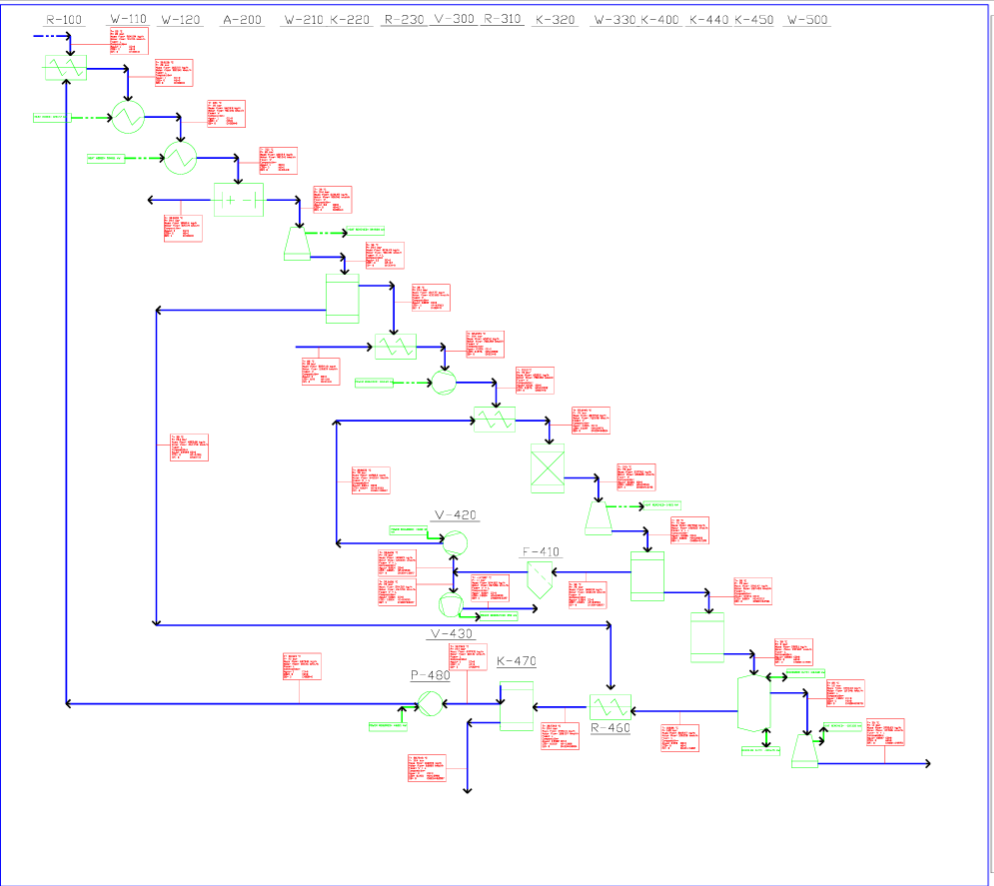
\includegraphics[width=0.98\textwidth,height=12.5cm,keepaspectratio]{figuras/dfp_plpl_1_1.png}
\caption{\textbf{Diagrama de Flujo de Proceso Preliminar (PFD v0 / DFP Solvanta PLPL 1.1)} -- Planta de e-Metanol Grado AA ($30\,000\text{ t/año}$). Archivo oficial: \texttt{03\_Entregables\_Finales/E1/VTP-01\_Solvanta/04\_PFD/PFD-v0\_Solvanta.pdf}.}
\end{figure}

\begin{center}
\footnotesize
\textbf{Notas Técnicas del Diagrama PFD v0:}
\begin{enumerate}[leftmargin=2.0em]
    \item La planta opera en régimen continuo con disponibilidad anual de $8\,000\text{ horas}$ ($91.3\%$ factor de servicio).
    \item El calor exotérmico de la síntesis de metanol en \texttt{R-401} ($9.14\text{ MW}$) se transfiere integralmente a la carcasa \texttt{E-201}, evaporando agua para alimentar la celda SOEC.
    \item La columna fraccionadora \texttt{T-701} opera con 28 platos reales y reflujo de $1.50$, garantizando pureza Grado AA ($\ge 99.85\%$ p/p húmedo, $100.00\%$ seco).
    \item El separador flash \texttt{V-801} desgasifica el agua residual antes de la bomba \texttt{P-801}, logrando vertido cero (ZLD) con reciclo total a SOEC.
\end{enumerate}
\end{center}

\clearpage

% ==============================================================================
% PÁGINA 14: LISTA DE VERIFICACIÓN DEL PFD Y ASUNTOS PENDIENTES
% ==============================================================================
\subsection{Lista de verificación del PFD v0}

\begin{center}
\footnotesize
\textbf{Cuadro 13: Lista de verificación cruzada del PFD v0.}\\[2pt]
\begin{tabularx}{\textwidth}{cp{8.2cm}cX}
\toprule
\textbf{Núm.} & \textbf{Criterio de Evaluación Técnica} & \textbf{Sí/No} & \textbf{Observación de la Firma Solvanta} \\
\midrule
1 & Todos los equipos principales están representados físicamente. & \textbf{Sí} & SOEC, BWR Lurgi, compresores, flashes, expansor y torre. \\
2 & Todos los equipos poseen identificador único estandarizado. & \textbf{Sí} & Tags coherentes según codificación del Cuadro 12. \\
3 & Las líneas cuentan con flechas de dirección de flujo. & \textbf{Sí} & Trazabilidad direccional continua sin ambigüedades. \\
4 & Todas las corrientes maestras se encuentran numeradas. & \textbf{Sí} & Numeración unívoca \texttt{S-01} a \texttt{S-16} y lazos ZLD. \\
5 & Los números de corriente coinciden al 100\% con TC-01. & \textbf{Sí} & Coincidencia cruzada perfecta verificada en Cuadro 9. \\
6 & Las cargas térmicas y potencias se localizan en TE-01. & \textbf{Sí} & Balances térmicos y potencias rotativas trazables. \\
7 & Entradas y productos comerciales plenamente identificados. & \textbf{Sí} & $\text{CO}_2$ captura, agua make-up, e-metanol y $\text{O}_2$. \\
8 & Purga continua del $4\%$ y recirculaciones representadas. & \textbf{Sí} & Lazo gas a C-601, purga a X-601 y agua ZLD a SOEC. \\
9 & Los bloques Recycle de DWSIM no aparecen como equipos. & \textbf{Sí} & Dibujados rigurosamente como líneas de tubería cerrada. \\
10 & El separador abstracto fue traducido a tecnología real. & \textbf{Sí} & Columna \texttt{T-701} de 28 platos y flash de efluentes \texttt{V-801}. \\
11 & Temperatura, presión y flujo coinciden con DWSIM v1. & \textbf{Sí} & Trazabilidad unívoca con caso aprobado congelado. \\
12 & Cajetín de ingeniería completo con fecha y revisión. & \textbf{Sí} & Cajetín Solvanta, RFP-CCM-EM-001, Rev. v0.1 Oficial. \\
13 & Calidad gráfica vectorial de alta legibilidad. & \textbf{Sí} & Renderizado de alta resolución con bloques de datos. \\
\bottomrule
\end{tabularx}
\end{center}

\vspace{0.4cm}
\subsection{Lista de asuntos pendientes para la siguiente etapa de diseño (E2)}

Para la continuidad inmediata del proyecto hacia el dimensionamiento y hojas de datos (Entregable E2):
\begin{enumerate}
    \item \textbf{Validación hidráulica de platos en T-701:} Ratificar el espaciado de platos ($0.50\text{ m}$) y diámetro preliminar ($1.25\text{ m}$) mediante análisis de inundación (flooding factor $<80\%$) y caída de presión en simulador hidráulico.
    \item \textbf{Cinética detallada en R-401:} Modelar el perfil de temperatura punto a punto en los tubos catalíticos con cinética de Vanden Bussche \& Froment en lugar de conversión pseudo-global.
    \item \textbf{Integración térmica avanzada (Pinch Analysis):} Evaluar la integración entre el efluente SOEC a $750^\circ\text{C}$ y el sobrecalentador de vapor \texttt{E-202} para reducir la demanda eléctrica neta de la planta.
    \item \textbf{Diseño mecánico de recipientes a presión:} Especificar metalurgia (acero inoxidable 316L y titanio) para los separadores flash y reactores que manejan $\text{CO}_2$ húmedo a alta presión.
\end{enumerate}

\clearpage

% ==============================================================================
% PÁGINA 15: PREGUNTAS TÉCNICAS DE CIERRE
% ==============================================================================
\section{Preguntas técnicas de cierre y evaluación de ingeniería}

\textbf{1. ¿Qué inconsistencias físicas o numéricas fueron detectadas durante la verificación de DWSIM v1?}\\
Se detectaron tres aspectos críticos: (a) En el lazo de reciclo de gas, el vapor de domo de \texttt{V-501} salía en su punto de rocío ($38^\circ\text{C}$), existiendo riesgo inminente de condensación y cavitación en el soplador \texttt{C-601}; (b) En la columna fraccionadora \texttt{T-701}, una sobre-especificación de flujo molar en el rehervidor provocaba incompatibilidad de balance de masa en el algoritmo Wang-Henke; y (c) El efluente acuoso se modelaba mediante un separador abstracto por componentes (\texttt{X-801}) carente de sentido físico industrial.

\textbf{2. ¿Cómo resolvió y documentó la firma Solvanta dichas inconsistencias?}\\
(a) Se incorporó el economizador gas-gas \texttt{E-601} ($272.05\text{ kW}$), sobrecalentando el gas de reciclo de $38^\circ\text{C}$ a $43^\circ\text{C}$ (vapor 100\% seco); (b) Se reconfiguraron las especificaciones de \texttt{T-701} a relación de reflujo ($1.50$) en el domo y recuperación de agua ($99.8\%$) en fondos, logrando convergencia directa en 2 iteraciones con Wang-Henke; y (c) Se reemplazó \texttt{X-801} por un recipiente flash adiabático vertical \texttt{V-801} a $19.4\text{ bar}$ conectado a la bomba \texttt{P-801}.

\textbf{3. ¿Qué dato del PFD v0 depende de un supuesto de ingeniería que aún debe validarse?}\\
La eficiencia global de platos de la columna \texttt{T-701} ($E_0 = 67.5\%$, equivalente a 28 platos reales frente a 19 platos teóricos) estimada mediante correlación general de O'Connell, la cual deberá validarse en la Etapa E2 mediante simulación de transferencia de masa Maxwell-Stefan.

\textbf{4. ¿Qué objeto de DWSIM requirió una traducción especial para representarse físicamente en el PFD v0?}\\
El reactor de síntesis de metanol: en DWSIM se modela mediante dos bloques vinculados (\texttt{R-401} cinético y \texttt{E-201} calentador acoplado), mientras que físicamente representa una sola unidad integrada: un reactor multitubular de lecho fijo tipo Lurgi (BWR) con tubos catalíticos cargados con $\text{Cu/ZnO/Al}_2\text{O}_3$ y carcasa generando vapor saturado a $20\text{ bar}$. Asimismo, los bloques \texttt{Recycle} se dibujaron como líneas cerradas de tubería.

\textbf{5. ¿Qué tecnología física se seleccionó para sustituir al separador abstracto por componentes?}\\
Se implementó una columna de destilación fraccionada rigurosa (\texttt{T-701}) de 28 platos reales con condensador total (\texttt{E-701}), acumulador de reflujo, rehervidor termosifón (\texttt{E-702}) y subenfriador de producto (\texttt{E-704}), complementada en los efluentes acuosos por el separador flash \texttt{V-801}.

\textbf{6. ¿Cuál es la principal pérdida de metanol identificada en el proceso y cuál es su magnitud?}\\
La principal pérdida ocurre como vapor arrastrado en la purga continua del bucle de síntesis (\texttt{S-13}) derivada hacia el turboexpansor \texttt{X-601}, cuantificada en $4.74\text{ kg/h}$ ($0.126\%$ de la producción horaria), complementada por trazas ínfimas en el venteo LP \texttt{V-701} ($0.88\text{ kg/h}$). La recuperación global de metanol en la planta es superior al $\mathbf{99.85\%}$.

\textbf{7. ¿Qué equipo presenta la mayor demanda energética y cuál es su participación relativa?}\\
El electrolizador cerámico de alta temperatura SOEC (\texttt{R-201} / \texttt{EL-201}), con una demanda de $54\,402.0\text{ kW}$ ($54.40\text{ MW}$ netos), representando el $\mathbf{98.37\%}$ del consumo eléctrico total de la planta para la disociación termoquímica de vapor a $750^\circ\text{C}$.

\textbf{8. ¿Qué equipos deberán dimensionarse prioritariamente en la siguiente etapa y por qué?}\\
El reactor multitubular \texttt{R-401} (gobierna la cinética de síntesis y la generación de vapor térmicamente integrada a la celda), el módulo SOEC \texttt{EL-201} (fija el área electroquímica, potencia eléctrica y suministro de $\text{H}_2$) y la columna \texttt{T-701} (asegura la especificación de pureza Grado AA del metanol).

\clearpage

% ==============================================================================
% PÁGINA 16: ESTRUCTURA DEL EXPEDIENTE Y FIRMAS DE APROBACIÓN
% ==============================================================================
\section{Estructura oficial del expediente digital (VTP-01\_Solvanta)}

La documentación técnica y archivos editables se encuentran estructurados en el repositorio oficial de GitHub (\href{https://github.com/karolcamachol29-sudo/RFP-CCM-EM-001}{\texttt{karolcamachol29-sudo/RFP-CCM-EM-001}}) bajo el siguiente árbol normalizado:

{\small
\begin{verbatim}
03_Entregables_Finales/E1/VTP-01_Solvanta/
|
|-- 01_DWSIM/
|   |-- DWSIM_v1_APROBADA_Solvanta.dwxmz    (Caso oficial congelado comprimido)
|   |-- DWSIM_v1_APROBADA_Solvanta.dwxml    (Archivo XML nativo legible)
|
|-- 02_Verificacion/
|   |-- Reporte_Verificacion.pdf            (Reporte detallado de corrida DWSIM)
|   |-- Evidencias/                         (Capturas de pantalla de convergencia)
|
|-- 03_Tablas/
|   |-- TC-01_Solvanta.pdf                  (Tabla oficial de corrientes de materia)
|   |-- TC-01_Solvanta.xlsx                 (Archivo editable de corrientes de materia)
|   |-- TE-01_Solvanta.pdf                  (Tabla oficial de energía y servicios)
|   |-- TE-01_Solvanta.xlsx                 (Archivo editable de balances térmicos)
|
|-- 04_PFD/
|   |-- PFD-v0_Solvanta.pdf                 (Diagrama de Flujo de Proceso exportado)
|   |-- PFD-v0_Solvanta.tex                 (Código fuente editable en LaTeX)
|   |-- PFD-v0_Solvanta_EDITABLE.pdf        (PDF editable para herramientas CAD)
|
|-- 05_Trazabilidad/
    |-- Matriz_Trazabilidad.pdf             (Matriz de consistencia cruzada DWSIM/PFD)
\end{verbatim}
}

\vspace{0.6cm}
\begin{center}
{\large \textbf{Firma y Validación Técnica del Entregable E1.5}}\\[0.2cm]
\small Solvanta Engineering Solutions S.A. de C.V. --- Proyecto Licitación RFP-CCM-EM-001
\end{center}

\vspace{0.8cm}
\begin{center}
\small
\begin{tabularx}{\textwidth}{YY}
\begin{center}
\underline{\makebox[6.5cm][c]{\textbf{Paulina Mota Macip}}} \\
\textbf{Responsable de Simulación DWSIM} \\
Ingeniería de Procesos Solvanta
\end{center}
&
\begin{center}
\underline{\makebox[6.5cm][c]{\textbf{Gildardo Ocaña Barrales}}} \\
\textbf{Responsable de PFD y Plant 3D} \\
Ingeniería de Diseño Mecánico Solvanta
\end{center}
\\[1.2cm]
\begin{center}
\underline{\makebox[6.5cm][c]{\textbf{Grecia Figueroa Rincón}}} \\
\textbf{Evaluación Económica \& HSE} \\
Análisis de Viabilidad y Sostenibilidad
\end{center}
&
\begin{center}
\underline{\makebox[6.5cm][c]{\textbf{Karol Paola Camacho López}}} \\
\textbf{Directora de Proyecto} \\
Optimización de Procesos y Gestión Técnica
\end{center}
\end{tabularx}
\end{center}

\vspace{0.6cm}
\begin{center}
\footnotesize
{\color{navyblue}\hrule height 0.8pt}
\vspace{0.2cm}
\textbf{Dictamen Docente DPyPQ:} Aprobado sin observaciones. El expediente técnico cumple la totalidad de criterios de convergencia, balances de materia sustituidos, pureza Grado AA, tablas TC-01/TE-01, PFD v0 y trazabilidad en GitHub.
\end{center}

\end{document}
